\documentclass[a4paper,twoside]{article}

% \VignetteIndexEntry{The htmf Package}
% \VignetteDepends{htmf}

\usepackage{fullpage}

\newcommand{\pkg}{\textbf}

\title{Overview of the \pkg{htmf} Package}
\author{Laurent Gautier <laurent@cbs.dtu.dk>\\
        <add your name here when adding content>}



\usepackage{Sweave}
\begin{document}

\maketitle

\section{Introduction}


\begin{Schunk}
\begin{Sinput}
> library(htmf)
\end{Sinput}
\end{Schunk}

The package \pkg{htmf} relies on other R packages:
\begin{Schunk}
\begin{Soutput}
[1] "reshape, ggplot2, Biobase, methods, stats"
\end{Soutput}
\end{Schunk}
Those must be available, or an error will occur when trying to attach \pkg{htmf}


\section{Reading data}

\subsection{Biolector}

The {\it biolector} system is recording the measurments in a CSV file.

The function \verb+read_biolector+ can be passed a filename or a connection
and read the file's content into a \verb+PlateRun+ data structure.

Here we use a {\it gzipped} connection:
\begin{Schunk}
\begin{Sinput}
> fn <- system.file("exampleData", "biolector_data.csv.gz", package="htmf")
> # Create a gzip connection
> gzf <- gzfile(fn)
> pr <- read_biolector(gzf)
> close(gzf)
\end{Sinput}
\end{Schunk}


\section{Plotting data}

\subsection{Default plots}
\begin{Schunk}
\begin{Sinput}
> # plot_biolector 
\end{Sinput}
\end{Schunk}

\subsection{Custom plots}

\begin{Schunk}
\begin{Sinput}
> dataf_biomass <- melt(measure(pr$Biomass))
> names(dataf_biomass)[ncol(dataf_biomass)] <- "biomass"
> p <- ggplot(dataf_biomass) +
+      aes(x = cycle, y = biomass) +
+      geom_line(aes(group = well), alpha = 0.3)
> print(p)
> 
\end{Sinput}
\end{Schunk}
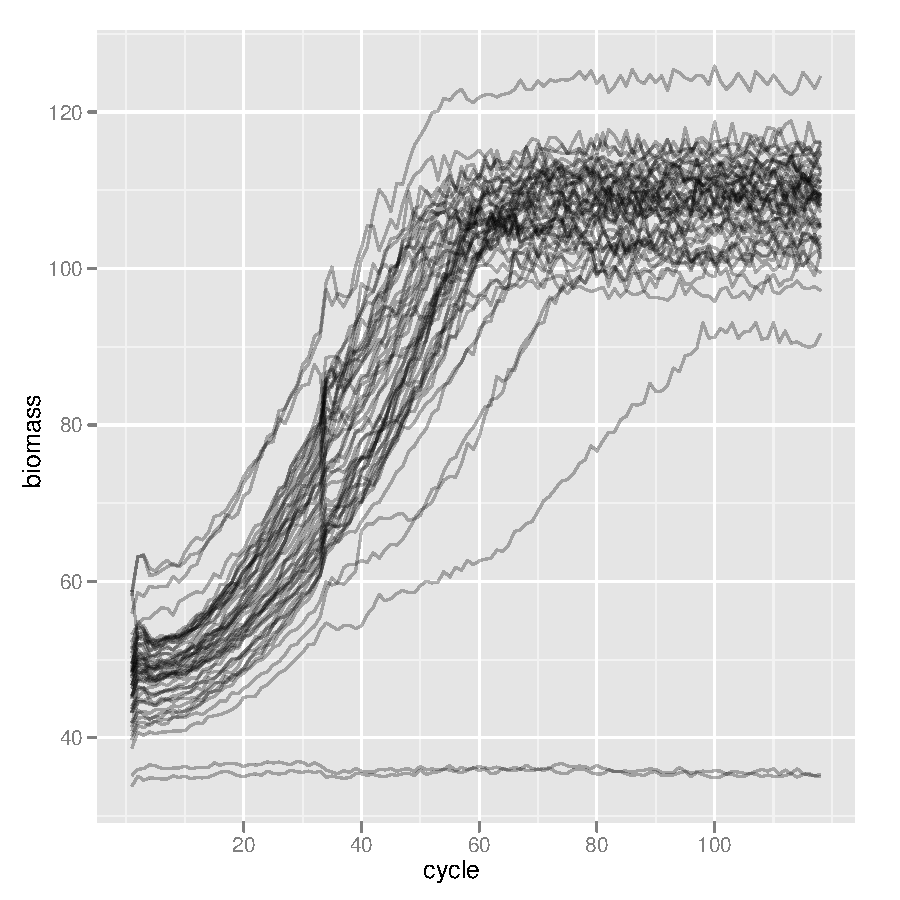
\includegraphics{htmf-005}

\begin{Schunk}
\begin{Sinput}
> p <- ggplot(subset(dataf_biomass, well %in% c("A01","B01","C01"))) +
+      aes(x = cycle, y = biomass, col = factor(well)) +
+      geom_smooth(aes(group = well), alpha = 0.3)
> print(p)
> 
\end{Sinput}
\end{Schunk}
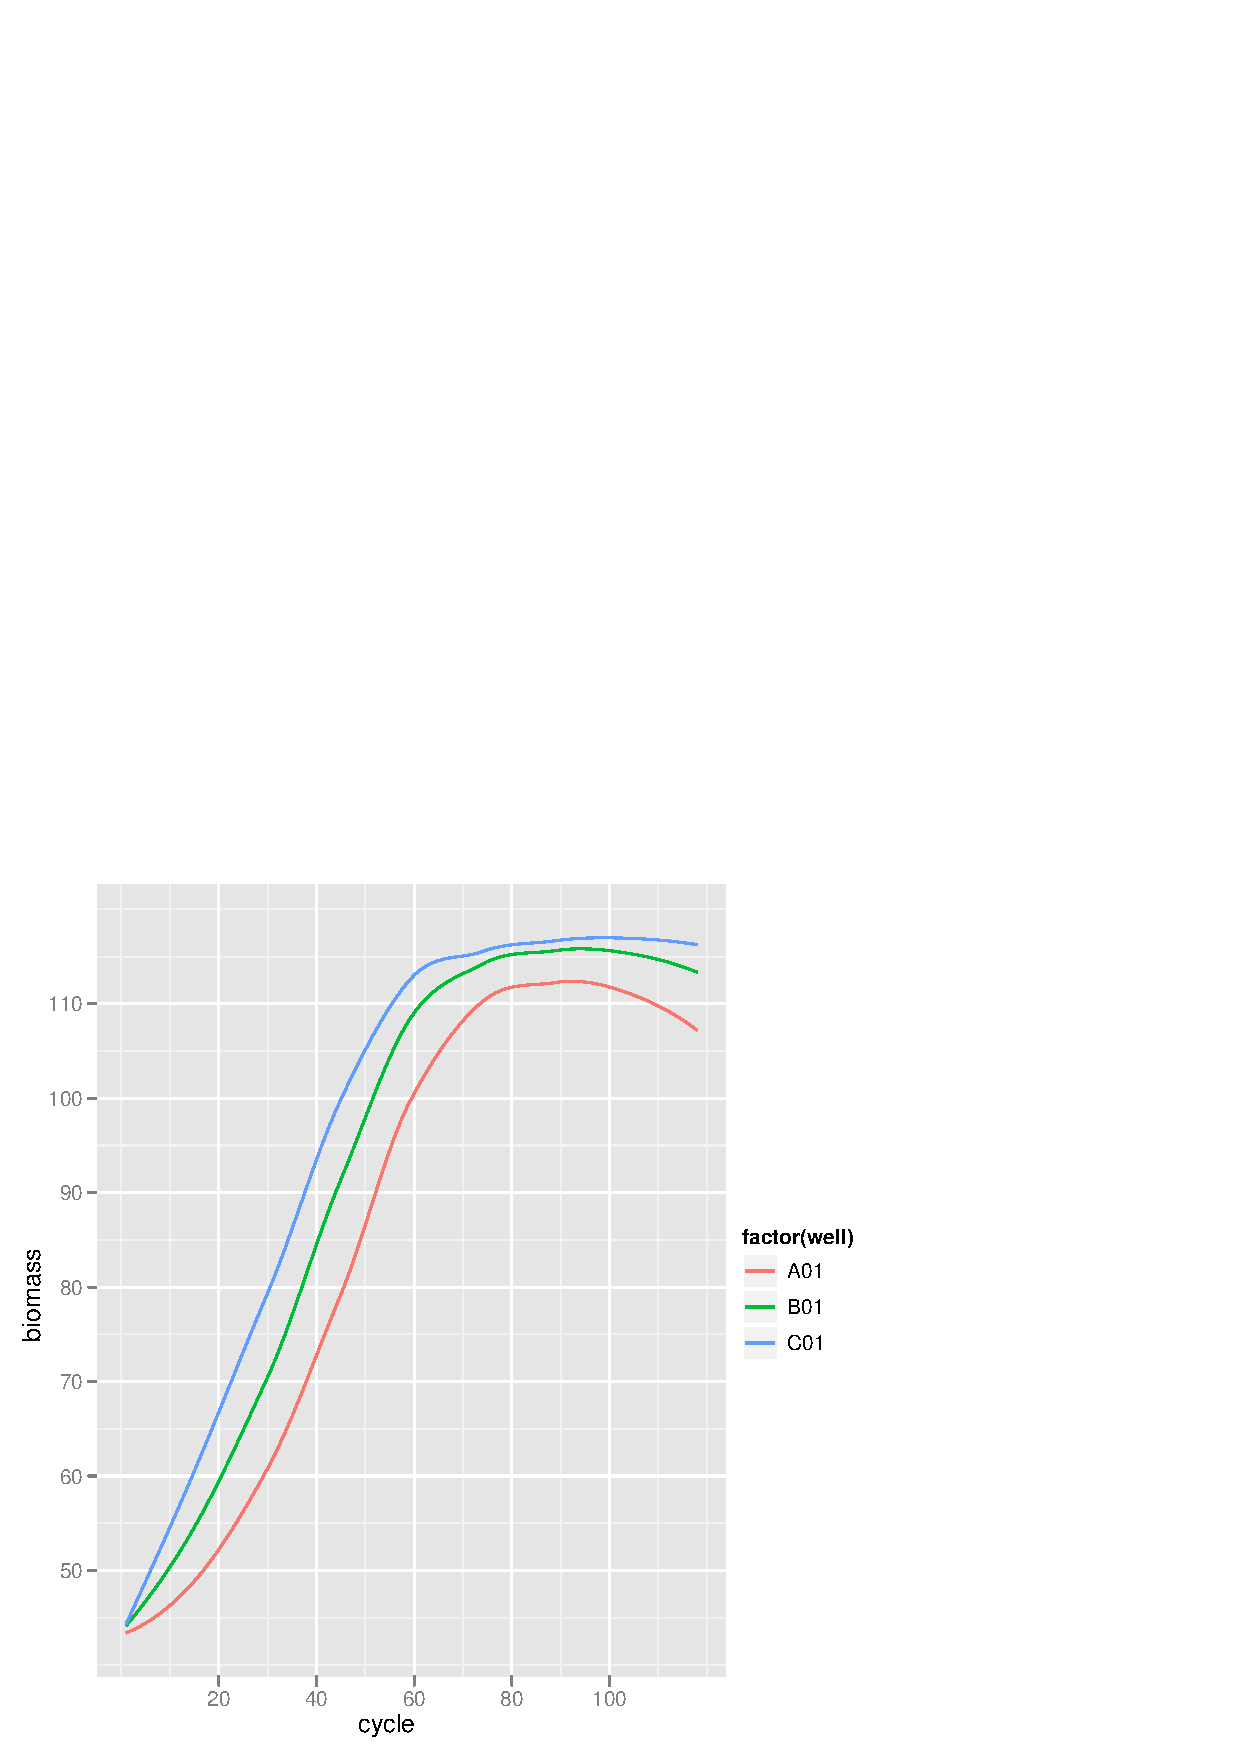
\includegraphics{htmf-006}


\section{Computing on the data}

\subsection{Adjusting the data}


\subsection{Fitting curves}

As observed in earlier plots of the biomass data, a logistic curve seems to be able to represent
our data. In an surprising move for fitting dose-respone or growth data, we choose the four-parameter logistic curve.

\[\mathnormal{response} = \mathnormal{f}(\mathnormal{input}) = A + \frac{ B - A }{ 1 + \exp(\frac{\mathnormal{xmid}-\mathnormal{input}}{\mathnormal{scal}})}\]

with
\begin{description}
\item[A: ] lower asymptote
\item[B: ] higher asymptote
\item[xmid: ] point of inflection
\item[scal: ] scale parameter
\end{description}
That function can be defined in R:
\begin{Schunk}
\begin{Sinput}
> fpl <- function(A, B, xmid, scal, x) A+(B-A)/(1+exp((xmid-x)/scal))
\end{Sinput}
\end{Schunk}

The first order derivative can be used to compute the slope at the inflection point:
\[\frac{d}{dx} f = \frac{B - A}{\mathnormal{scal} (1+\exp(\frac{m-\mathnormal{x}}{\mathnormal{scal}}))^2} \]




The package \pkg{nlme} is used for the fitting, and to demonstrate how to do it only one growth curve is worked on.
\begin{Schunk}
\begin{Sinput}
> library(nlme)
> dataf_wells <- split(dataf_biomass, dataf_biomass$well)
> params <- getInitial(biomass ~ SSfpl(cycle, 110, 0, 0, 0), 
+                      data=dataf_wells[[1]])
> params
\end{Sinput}
\begin{Soutput}
       110          0          0          0 
 46.219825 110.889552  44.368340   8.776391 
\end{Soutput}
\begin{Sinput}
> A <- params[1]; B <- params[2]
> xmid <- params[3]; scal <- params[4]
> fit <- nls(biomass ~ SSfpl(cycle, A, B, xmid, scal), 
+            alg="plinear", data=dataf_wells[[1]])
> fit
\end{Sinput}
\begin{Soutput}
Nonlinear regression model
  model:  biomass ~ SSfpl(cycle, A, B, xmid, scal) 
   data:  dataf_wells[[1]] 
      A       B    xmid    scal    .lin 
 46.220 110.890  44.368   8.776   1.000 
 residual sum-of-squares: 377.9

Number of iterations to convergence: 0 
Achieved convergence tolerance: 2.852e-14 
\end{Soutput}
\end{Schunk}


The estimated parameters can be related to physical or biological representations with
\begin{description}
  \item[A:] amount of cells inoculated
  \item[B:] amount of cells at the end of the fermentation
  \item[slope at the inflection point:] maximum growth
\end{description}
as shown on the figure below.

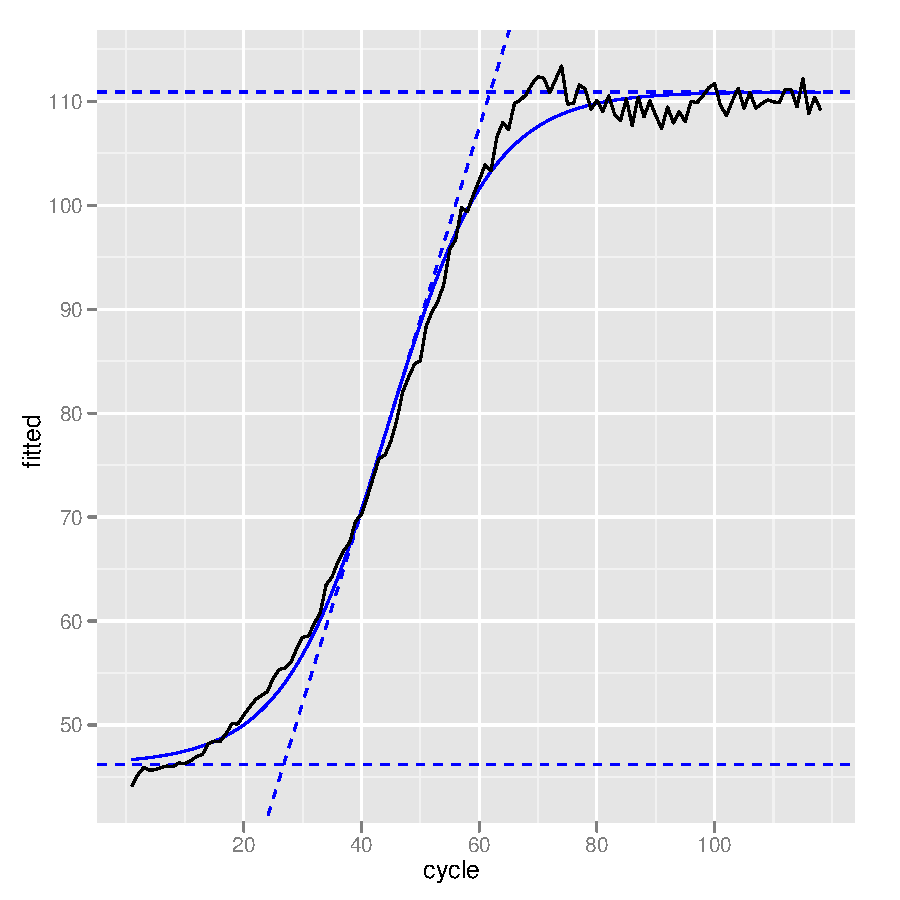
\includegraphics{htmf-010}

% guts feeling that it is wrong (done in a rush with very rusty derivation skills) -LG



This process can be automated, and parameters of growth fitted without the user's assistance.

\begin{Schunk}
\begin{Sinput}
> for (i in 1:20) {
+ 
+   params <- tryCatch(getInitial(biomass ~ SSfpl(cycle, 110, 0, 0, 0), 
+                                 data=dataf_wells[[i]]),
+                      error = function(e) NULL)
+   if (is.null(params)) {
+     dataf_wells[[i]]$fitted <- rep(NA, length = nrow(dataf_wells[[i]]))
+   } else {
+     A <- params[1]; B <- params[2]
+     xmid <- params[3]; scal <- params[4]
+     fit <- nls(biomass ~ SSfpl(cycle, A, B, xmid, scal), alg="plinear", 
+                data=dataf_wells[[i]])
+ 
+     tmp <- coef(fit)
+     dataf_wells[[i]]$fitted <- fpl(tmp[1], tmp[2], tmp[3], tmp[4], 
+                                    dataf_wells[[i]]$cycle)
+   }
+ }
> dataf_ten <- do.call("rbind", dataf_wells[1:20])
> p <- ggplot(dataf_ten) +
+      geom_line(aes(x = cycle, y = biomass), col="black") +
+      geom_line(aes(x = cycle, y = fitted), col="blue", linetype = 2) +
+      facet_wrap( ~ well)
> print(p)
> 
\end{Sinput}
\end{Schunk}
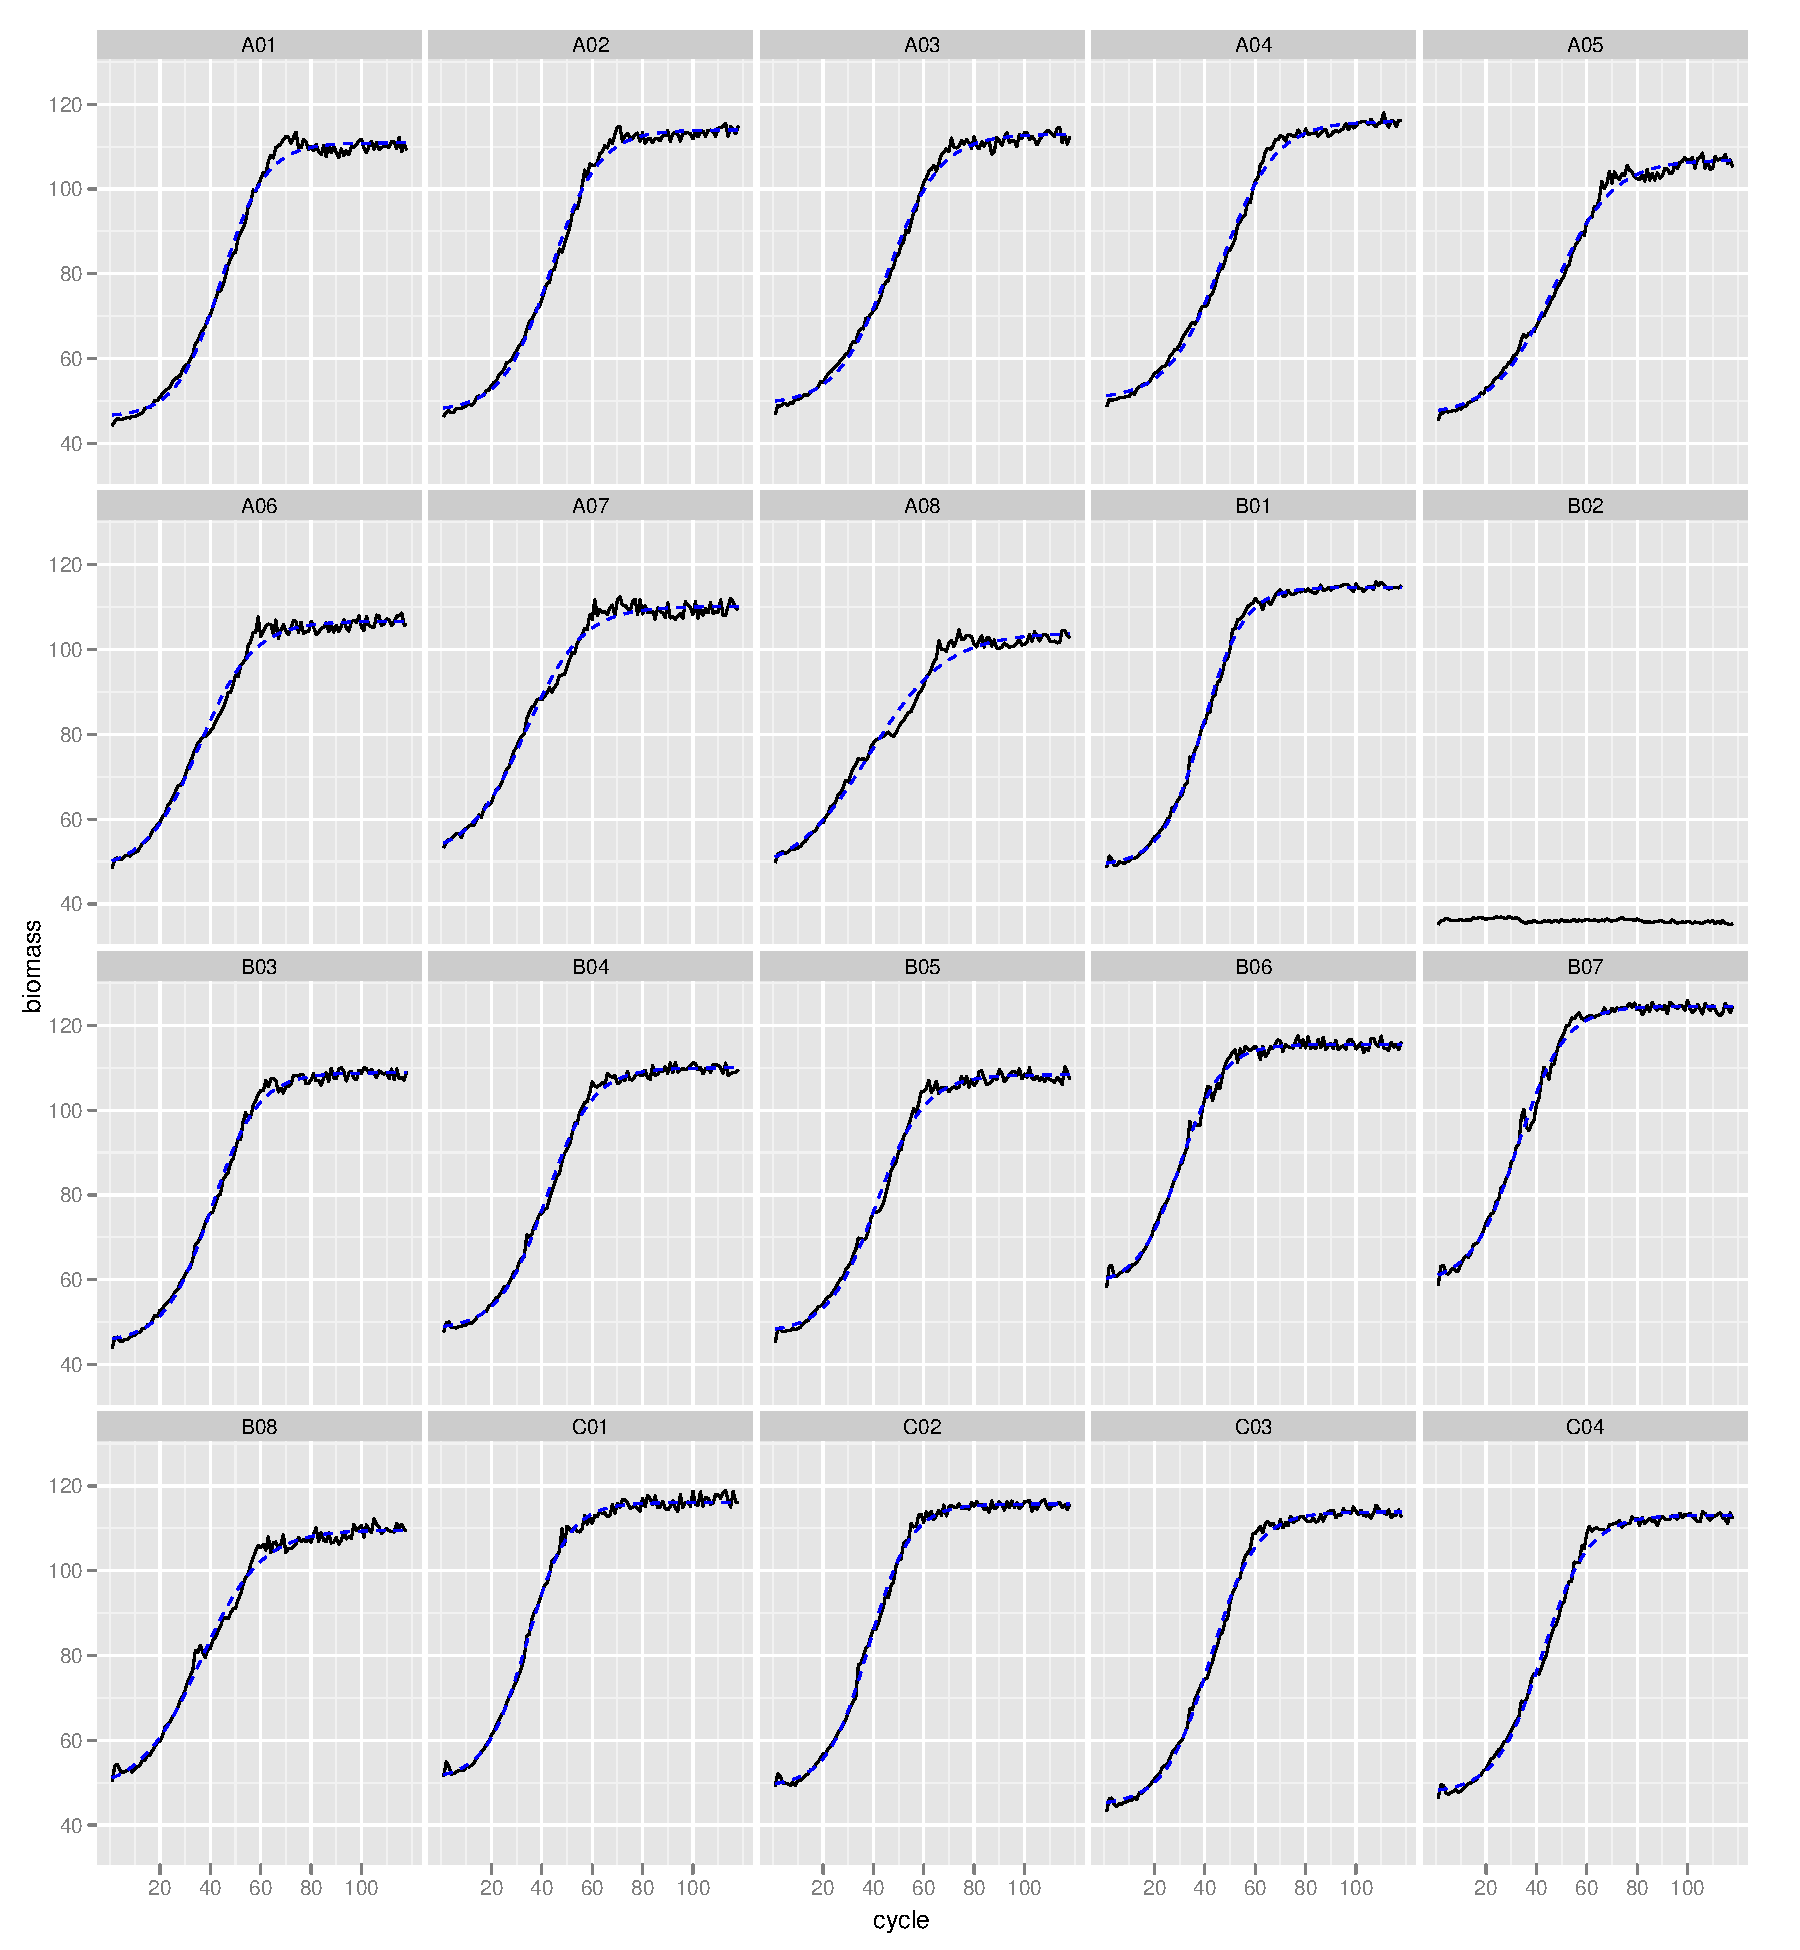
\includegraphics{htmf-012}


\end{document}

